% Native PGFPlots; generated by examples/generate_figures.py.
% Constructed or analytical teaching example.
\begingroup
\definecolor{blueplot}{HTML}{4E79A7}
\definecolor{redplot}{HTML}{D95F59}
\definecolor{inkplot}{HTML}{111111}
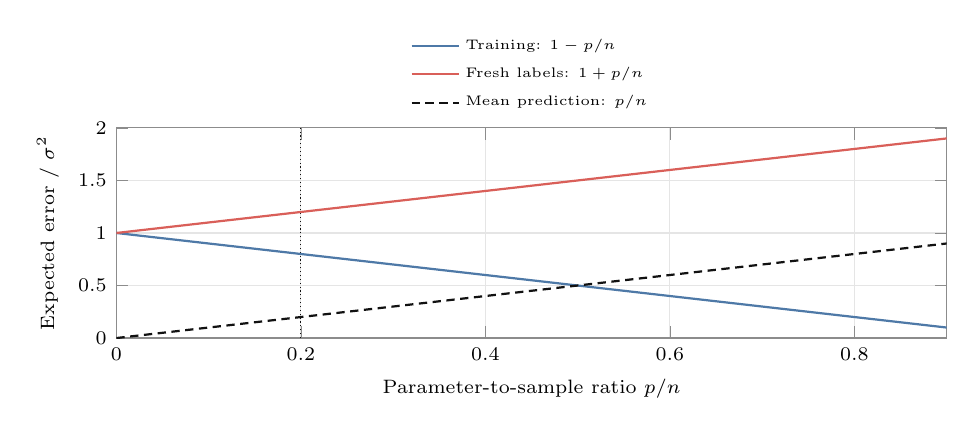
\begin{tikzpicture}
\begin{axis}[
width=\linewidth,height=4.25cm,font=\scriptsize,
tick label style={font=\scriptsize},label style={font=\scriptsize},
axis line style={black!45},tick style={black!45},
grid=major,grid style={black!10},scaled ticks=false,
clip=true,unbounded coords=jump,
legend style={font=\tiny,draw=none,fill=white,fill opacity=.94,text opacity=1,
  legend cell align=left,inner sep=2pt,row sep=1pt},
xmin=0,xmax=.9,ymin=0,ymax=2,
xlabel={Parameter-to-sample ratio $p/n$},ylabel={Expected error / $\sigma^2$},
xtick={0,.2,.4,.6,.8},ytick={0,.5,1,1.5,2},
legend style={at={(.5,1.03)},anchor=south}
]
\addplot[inkplot,densely dotted,forget plot] coordinates {(.2,0) (.2,2)};
\addplot[blueplot,thick,no marks,domain=0:.9] {1-x};
\addlegendentry{Training: $1-p/n$}
\addplot[redplot,thick,no marks,domain=0:.9] {1+x};
\addlegendentry{Fresh labels: $1+p/n$}
\addplot[inkplot,thick,densely dashed,no marks,domain=0:.9] {x};
\addlegendentry{Mean prediction: $p/n$}

\end{axis}
\end{tikzpicture}
\endgroup
